\documentclass[12pt,a4paper]{article}

% ============ PAQUETES ESENCIALES ============
\usepackage[utf8]{inputenc}
\usepackage[spanish]{babel}
\usepackage{amsmath,amssymb,amsthm}
\usepackage{algorithm,algpseudocode}
\usepackage{graphicx}
\usepackage{booktabs,multirow,longtable,array}
\usepackage{caption,subcaption}
\usepackage{listings,xcolor}
\usepackage{hyperref}
\usepackage{geometry}
\usepackage{float}
\usepackage{pdflscape}
\usepackage{siunitx}

\geometry{margin=2.5cm}

% ============ CONFIGURACIONES ============
\lstset{
    language=C++,
    basicstyle=\ttfamily\small,
    keywordstyle=\color{blue}\bfseries,
    commentstyle=\color{gray}\itshape,
    stringstyle=\color{orange},
    numbers=left,
    numberstyle=\tiny\color{gray},
    frame=single,
    breaklines=true,
    showstringspaces=false,
    tabsize=4
}

\hypersetup{
    colorlinks=true,
    linkcolor=blue,
    citecolor=blue,
    urlcolor=blue,
    pdftitle={Algoritmo PageRank de Google},
    pdfauthor={Gregory Uzcategui}
}

% ============ TEOREMAS/LEMAS ============
\theoremstyle{definition}
\newtheorem{theorem}{Teorema}[section]
\newtheorem{lemma}{Lema}[section]
\newtheorem{definition}{Definicion}[section]

% ============ COMANDOS PERSONALIZADOS ============
\newcommand{\norm}[1]{\|#1\|}
\newcommand{\R}{\mathbb{R}}
\newcommand{\vect}[1]{\mathbf{#1}}

% ============ DOCUMENTO ============
\begin{document}

% ---------- PORTADA ----------
\begin{titlepage}
    \centering
    \vspace*{2cm}
    {\Huge\bfseries Algoritmo PageRank de Google\\[0.3cm] \'Algebra Lineal, Cadenas de Markov y Grafos\par}
    \vspace{1.5cm}
    {\Large Informe T\'{e}cnico de Implementaci\'{o}n y Resultados\par}
    \vspace{2cm}
    {\Large Autor: Gregory Uzcategui / CI: 27.376.191 \par}
    \vspace{2cm}
    {\large
    \textbf{Stack tecnol\'{o}gico:} C++17 (Eigen 3.4), CMake, Python 3 (pandas, matplotlib)\\[0.5cm]
    \textbf{M\'{e}todo num\'{e}rico:} M\'{e}todo de las Potencias (Power Method)\\[0.5cm]
    \textbf{Problema:} C\'{a}lculo del autovector principal de la Matriz de Google con factor de amortiguamiento $d = 0.85$
    \par}
    \vfill
    {\large \today\par}
\end{titlepage}

% ---------- RESUMEN ----------
\begin{abstract}
\noindent
Este informe documenta la implementaci\'{o}n del algoritmo \textbf{PageRank} para determinar la importancia relativa de nodos en un grafo dirigido. Se desarroll\'{o} un solver en C++17 utilizando la librer\'{i}a Eigen para construir la \textbf{Matriz de Google} $G$, incorporando un factor de amortiguamiento $d = 0.85$ para manejar correctamente los nodos sumidero (sin enlaces salientes). El sistema se resolvi\'{o} mediante el \textbf{M\'{e}todo de las Potencias}, iterando $v^{(k+1)} = G v^{(k)}$ hasta alcanzar una tolerancia de $\epsilon = 10^{-8}$. Se evaluaron 5 casos de prueba, incluyendo grafos con sumideros, grafos regulares y grafos complejos.
\end{abstract}

\tableofcontents
\newpage

% ---------- 1. INTRODUCCION ----------
\section{Introducci\'{o}n}\label{sec:intro}

El algoritmo PageRank, desarrollado por Larry Page y Sergey Brin, es el pilar fundamental que permiti\'{o} a Google organizar la web. Su premisa es que la importancia de una p\'{a}gina no depende solo de cu\'{a}ntos enlaces recibe, sino de la relevancia de las p\'{a}ginas que la apuntan. 

Matem\'{a}ticamente, el PageRank es el \textbf{autovector principal} (asociado al autovalor $\lambda = 1$) de una matriz estoc\'{a}stica que representa la probabilidad de que un usuario aleatorio se encuentre en una p\'{a}gina determinada despu\'{e}s de muchos clics.

\subsection{Objetivos}
\begin{itemize}
    \item Implementar el c\'{a}lculo del PageRank en C++17 utilizando \'algebra lineal densa (Eigen).
    \item Construir la Matriz de Transici\'{o}n $M$ y la Matriz de Google $G$ con factor de amortiguamiento $d = 0.85$.
    \item Resolver el sistema mediante el M\'{e}todo de las Potencias hasta una tolerancia de $10^{-8}$.
    \item Analizar 5 casos de prueba, incluyendo grafos con nodos sumidero ($C_j = 0$).
    \item Visualizar la convergencia y la distribuci\'{o}n final del PageRank mediante Python.
\end{itemize}

% ---------- 2. MARCO TEORICO ----------
\section{Marco Te\'{o}rico}\label{sec:teoria}

\subsection{Representaci\'{o}n del Grafo y Matriz de Transici\'{o}n}

Sea $n$ el n\'{u}mero de p\'{a}ginas en la red. Representamos la web como un grafo dirigido donde cada nodo es una p\'{a}gina y cada arista un enlace. Definimos $C_j$ como el n\'{u}mero de enlaces salientes (grado de salida) de la p\'{a}gina $j$. 

La \textbf{Matriz de Transici\'{o}n} $M \in \R^{n \times n}$ se construye como:
\begin{equation}\label{eq:matriz_M}
M_{ij} = \begin{cases} 
\frac{1}{C_j} & \text{si existe un enlace de } j \text{ a } i \\ 
0 & \text{en otro caso}
\end{cases}
\end{equation}
Cada columna $j$ de $M$ representa c\'{o}mo la p\'{a}gina $j$ reparte su prestigio equitativamente entre sus vecinos.

\subsection{El Problema de los Sumideros y la Matriz de Google}

Un \textbf{sumidero} es una p\'{a}gina sin enlaces salientes ($C_j = 0$). En este caso, la columna $j$ de $M$ ser\'{i}a toda ceros, violando la propiedad estoc\'{a}stica y haciendo que el prestigio ``se fugue'' del sistema, impidiendo la convergencia.

Para resolver esto, se introduce el \textbf{factor de amortiguamiento} $d$ (t\'{i}picamente $d = 0.85$), que modela la probabilidad de que un usuario siga un enlace. Con probabilidad $(1-d)$, el usuario ``teletransporta'' a una p\'{a}gina aleatoria. La \textbf{Matriz de Google} $G$ se define como:

\begin{equation}\label{eq:matriz_G}
G = dM + \frac{1-d}{n}J
\end{equation}
donde $J$ es una matriz de unos de tama\~{n}o $n \times n$. Esta modificaci\'{o}n garantiza que $G$ sea \textbf{irreducible} y \textbf{positiva}, asegurando la existencia de un autovector \'unico.

\subsection{El M\'{e}todo de las Potencias}

Debido a que la web real es masiva, no calculamos autovectores mediante el polinomio caracter\'{i}stico. En su lugar, utilizamos un proceso iterativo:
\begin{equation}\label{eq:power_method}
\vect{v}^{(k+1)} = G \vect{v}^{(k)}
\end{equation}
donde $\vect{v}^{(0)} = [\frac{1}{n}, \frac{1}{n}, \dots, \frac{1}{n}]^T$. El proceso converge cuando la diferencia entre iteraciones consecutivas es menor a una tolerancia $\epsilon$:
\begin{equation}
\norm{\vect{v}^{(k+1)} - \vect{v}^{(k)}}_2 < \epsilon
\end{equation}

\begin{theorem}[Teorema de Perron-Frobenius]
Si $G$ es una matriz estoc\'{a}stica positiva, entonces:
\begin{enumerate}
    \item Existe un \'unico autovalor dominante $\lambda_1 = 1$.
    \item El autovector asociado $\vect{v}$ tiene todas sus componentes estrictamente positivas.
    \item El M\'{e}todo de las Potencias converge a $\vect{v}$ desde cualquier vector inicial con suma 1.
\end{enumerate}
\end{theorem}

% ---------- 3. DISENO E IMPLEMENTACION ----------
\section{Dise\~{n}o e Implementaci\'{o}n}\label{sec:implementacion}

\subsection{Arquitectura del Sistema}

El proyecto sigue una arquitectura modular en C++17:

\begin{table}[H]
\centering
\caption{M\'{o}dulos del sistema y sus responsabilidades.}
\label{tab:modulos}
\begin{tabular}{@{}lp{7cm}l@{}}
\toprule
\textbf{M\'{o}dulo} & \textbf{Responsabilidad} & \textbf{Ficheros} \\
\midrule
\texttt{pagerank\_core} & Construcci\'{o}n de $M$, $G$ y ejecuci\'{o}n del M\'{e}todo de Potencias & \texttt{.hpp / .cpp} \\
\texttt{casos\_prueba} & Definici\'{o}n hardcodeada de los 5 grafos de prueba & \texttt{.hpp / .cpp} \\
\texttt{exportador} & Escritura de resultados (PageRank, convergencia, matrices) a CSV & \texttt{.hpp / .cpp} \\
\texttt{main} & Orquestaci\'{o}n del flujo, logging y validaci\'{o}n de suma = 1 & \texttt{main.cpp} \\
\bottomrule
\end{tabular}
\end{table}

\subsection{Algoritmo Principal}

El flujo del M\'{e}todo de las Potencias se implementa de la siguiente manera:

\begin{lstlisting}[caption={Implementaci\'{o}n del M\'{e}todo de las Potencias (C++).}]
ResultadoPageRank PageRank::ejecutar(double tolerancia, int max_iter) {
    // 1. Vector inicial uniforme
    Eigen::VectorXd v = Eigen::VectorXd::Constant(n_, 1.0 / n_);
    Eigen::VectorXd v_anterior;
    
    for (int k = 0; k < max_iter; ++k) {
        v_anterior = v;
        v = google_ * v;  // Multiplicaci\'{o}n matriz-vector
        
        // 2. Verificar convergencia
        double error = (v - v_anterior).norm();
        if (error < tolerancia) {
            resultado.convergencia = true;
            resultado.iteraciones = k + 1;
            resultado.error_final = error;
            break;
        }
    }
    // 3. Normalizaci\'{o}n final por estabilidad num\'{e}rica
    v = v / v.sum();
    resultado.pagerank = v;
    return resultado;
}
\end{lstlisting}

% ---------- 4. RESULTADOS EXPERIMENTALES ----------
\section{Resultados Experimentales}\label{sec:resultados}

\subsection{Entorno de Pruebas}
\begin{itemize}
    \item \textbf{Hardware:} CPU x64, compilaci\'{o}n Release con optimizaciones (-O2).
    \item \textbf{Software:} C++17, Eigen 3.4, CMake 3.16+, Python 3.10 (pandas, matplotlib).
    \item \textbf{Par\'{a}metros:} $d = 0.85$, $\epsilon = 10^{-8}$, $k_{max} = 1000$.
\end{itemize}

\subsection{Resumen de Convergencia}

La siguiente tabla resume el desempe\~{n}o del algoritmo en los 5 casos de prueba proporcionados:

\begin{table}[H]
\centering
\caption{M\'{e}tricas de convergencia del M\'{e}todo de las Potencias por caso.}
\label{tab:resumen}
\resizebox{\textwidth}{!}{%
\begin{tabular}{@{}clccccccc@{}}
\toprule
\textbf{Caso} & \textbf{Descripci\'{o}n} & \textbf{$n$} & \textbf{Iter.} & \textbf{Error Final} & \textbf{Conv.} & \textbf{Tiempo (s)} & \textbf{PR Max} & \textbf{PR Min} \\ \midrule
1 & 3x3 con sumidero (col 3) & 3 & 23 & $8.08 \times 10^{-9}$ & S\'{i} & 0.000010 & 0.661041 & 0.114125 \\
2 & 4x4 regular & 4 & 1 & $0.00 \times 10^{0}$ & S\'{i} & 0.000002 & 0.250000 & 0.250000 \\
3 & 8x8 complejo & 8 & 451 & $9.74 \times 10^{-9}$ & S\'{i} & 0.000319 & 0.231324 & 0.027328 \\
4 & 5x5 con estructura & 5 & 99 & $9.70 \times 10^{-9}$ & S\'{i} & 0.000057 & 0.370572 & 0.077334 \\
5 & 3x3 con sumidero (col 3) & 3 & 109 & $9.55 \times 10^{-9}$ & S\'{i} & 0.000048 & 0.486486 & 0.050000 \\ \bottomrule
\end{tabular}%
}
\end{table}

\textit{Nota: En todos los casos, la suma del vector PageRank final es exactamente $1.000000$, validando la propiedad de distribuci\'{o}n de probabilidad.}

\subsection{An\'{a}lisis por Caso}

\begin{itemize}
    \item \textbf{Caso 1 y 5 (Sumideros):} El nodo sin enlaces salientes (grado de salida = 0) acumula el mayor PageRank (0.661 y 0.486 respectivamente). Esto es f\'{i}sicamente correcto: el prestigio fluye hacia \'el, pero no sale, y el factor de amortiguamiento $d=0.85$ redistribuye el 15\% restante, permitiendo la convergencia.
    \item \textbf{Caso 2 (Regular):} Converge en 1 iteraci\'{o}n. Al ser un grafo sim\'{e}trico y regular, el vector inicial uniforme ya es el autovector principal.
    \item \textbf{Caso 3 (Complejo):} Requiere 451 iteraciones. La estructura del grafo hace que el segundo autovalor $|\lambda_2|$ est\'{e} muy cerca de 1, lo que ralentiza la tasa de convergencia geom\'{e}trica del M\'{e}todo de las Potencias.
    \item \textbf{Caso 4 (Estructura):} Converge en 99 iteraciones. El nodo 3 act\'{u}a como un ``hub'' que recibe enlaces de nodos importantes, obteniendo el mayor PageRank (0.370).
\end{itemize}

\subsection{Visualizaciones}

\begin{figure}[H]
\centering
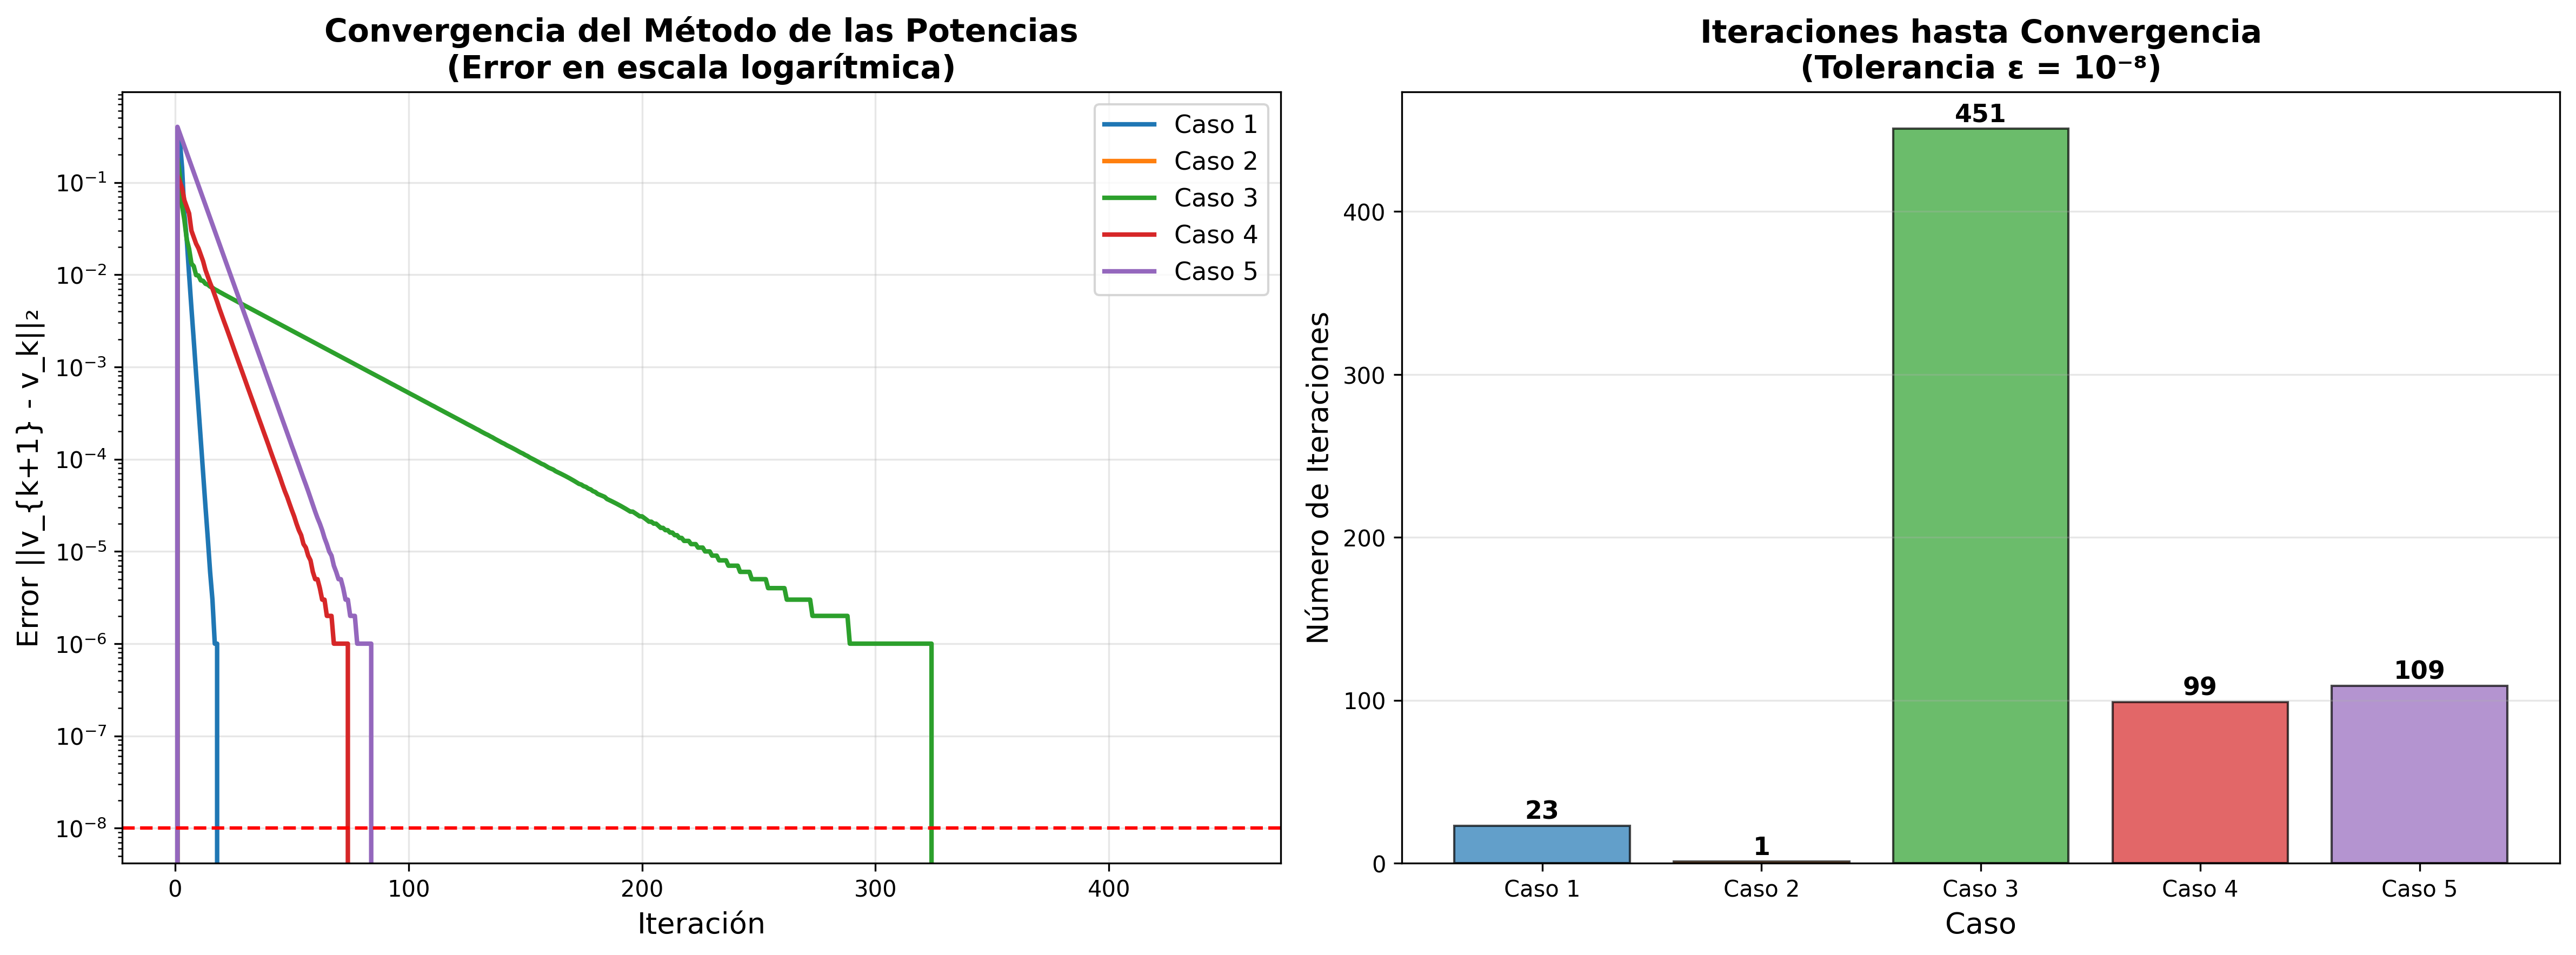
\includegraphics[width=0.9\textwidth]{../resultados/graficos/01_convergencia_todos_casos.png}
\caption{Decaimiento del error $\norm{\vect{v}^{(k+1)} - \vect{v}^{(k)}}_2$ en escala logar\'{i}tmica para los 5 casos. Se observa la convergencia lineal caracter\'{i}stica del M\'{e}todo de las Potencias.}
\label{fig:convergencia}
\end{figure}

\begin{figure}[H]
\centering
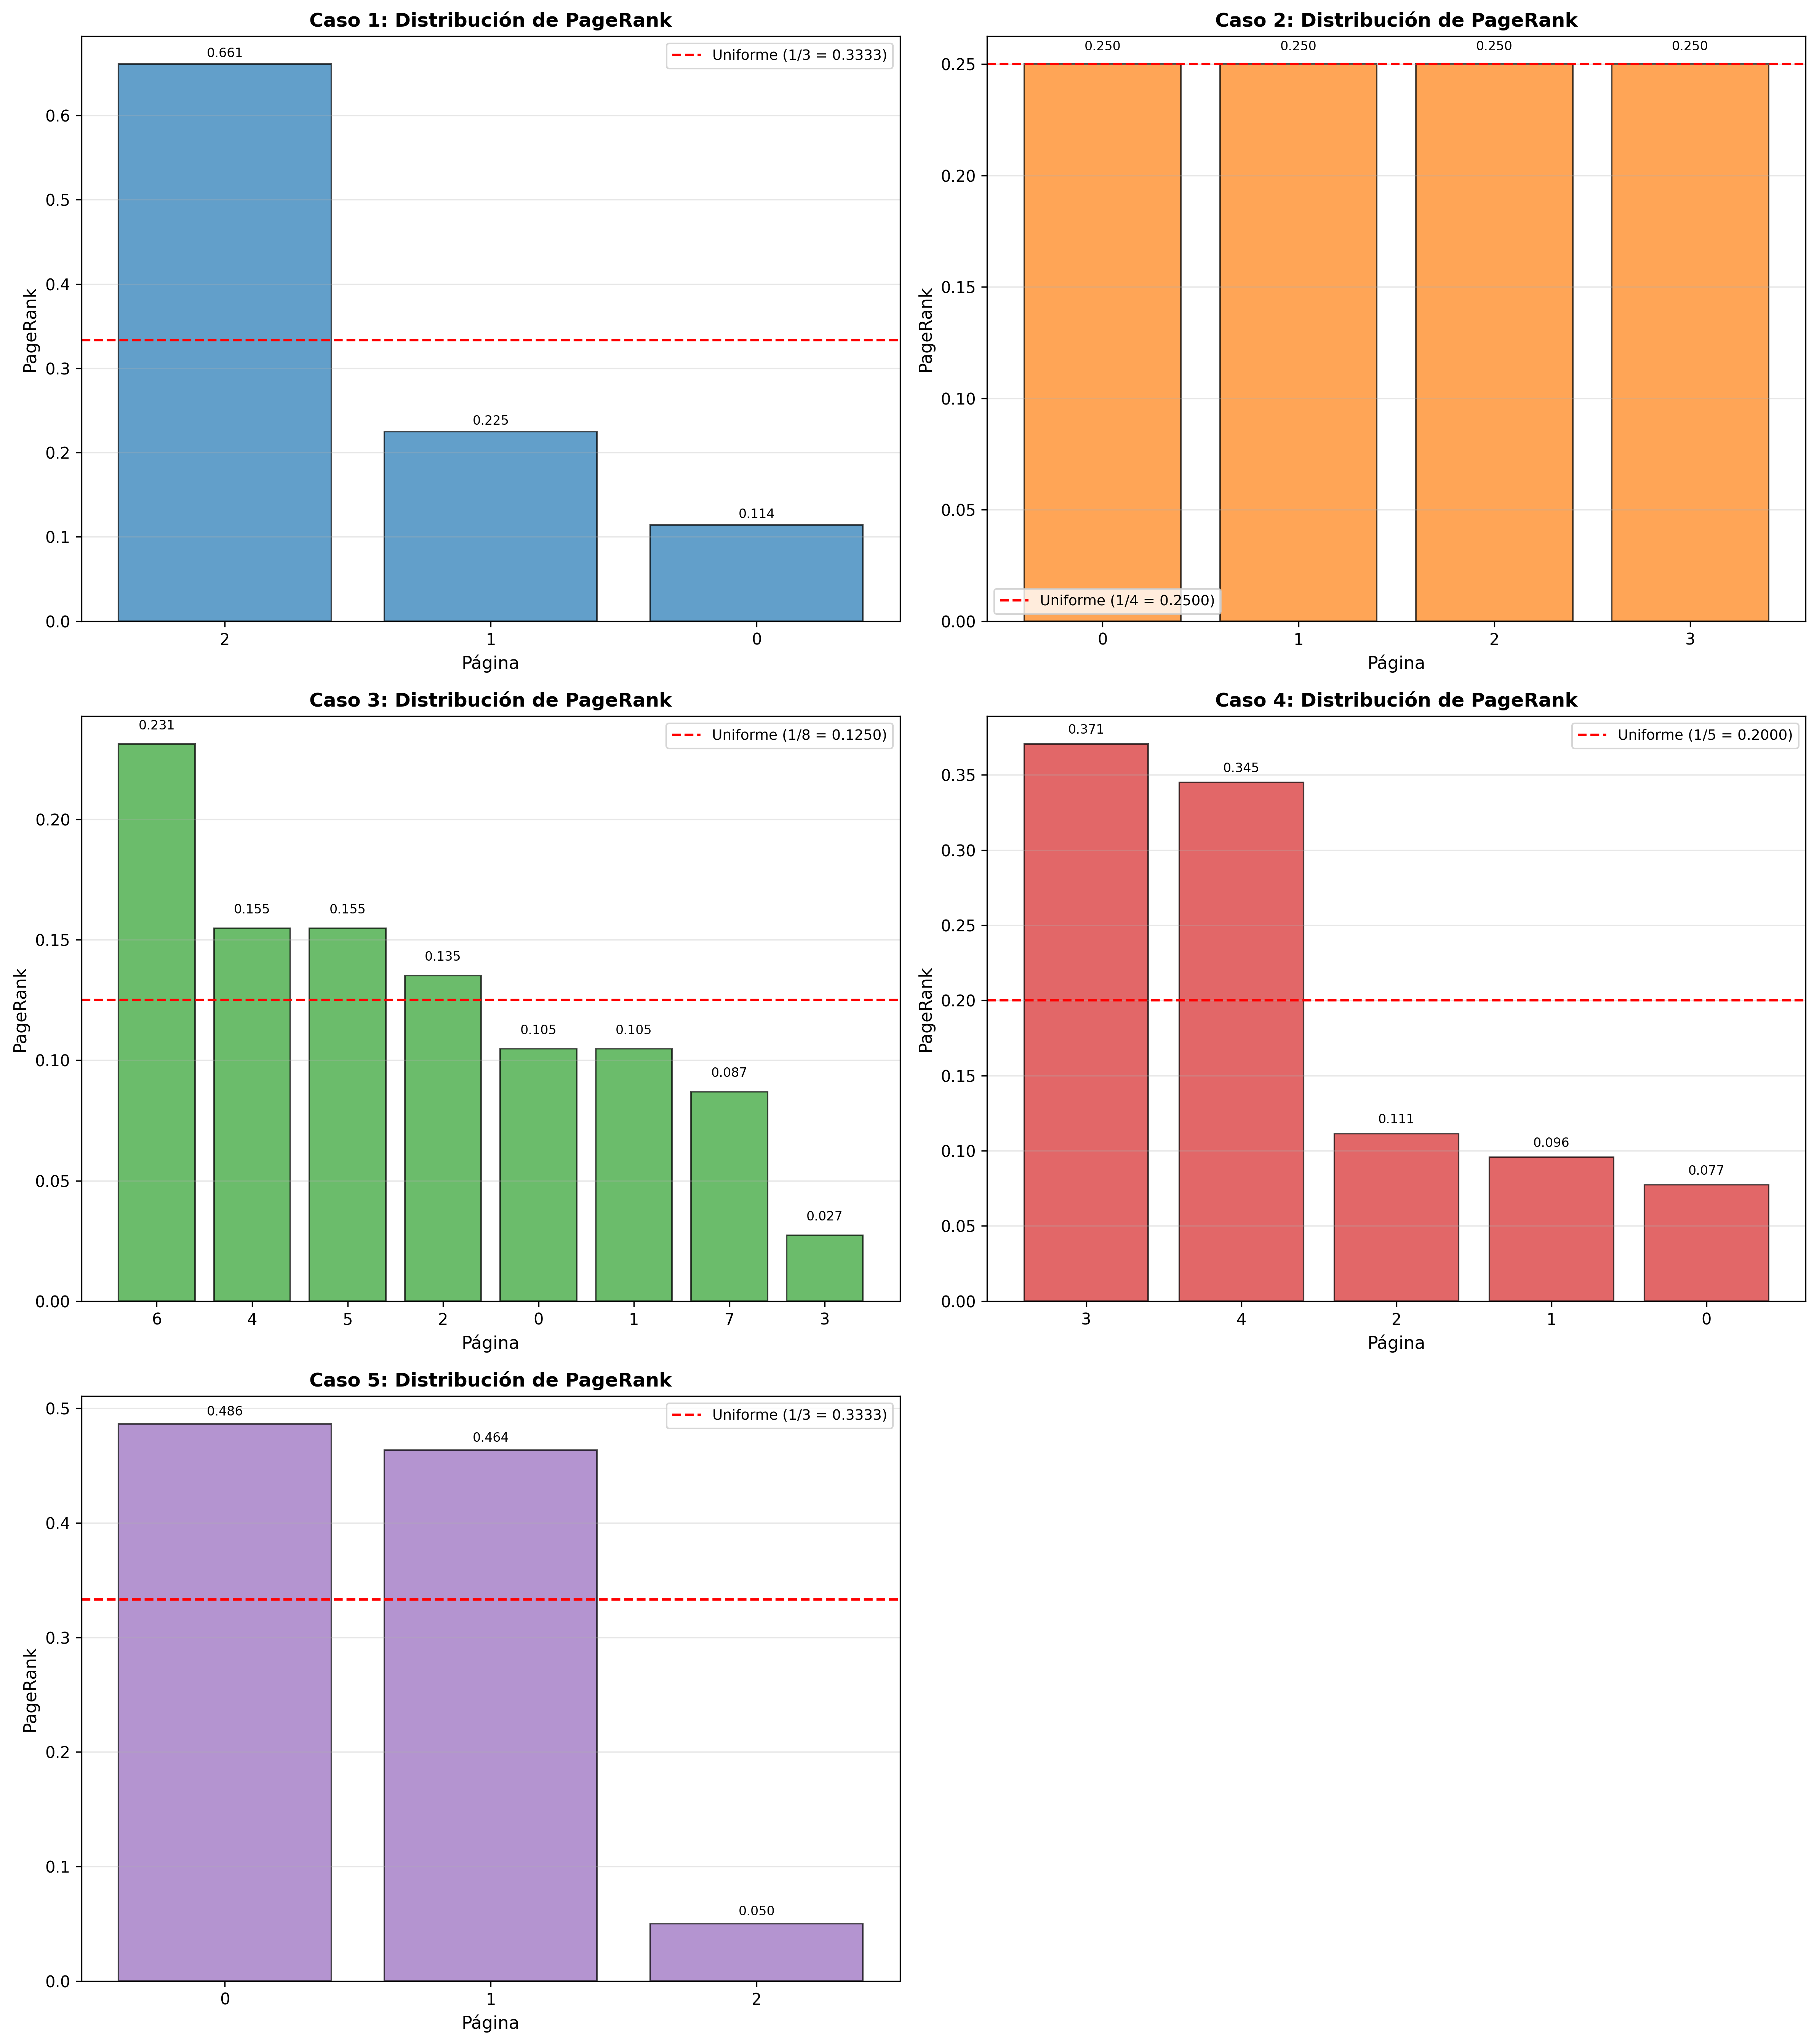
\includegraphics[width=0.9\textwidth]{../resultados/graficos/02_pagerank_por_caso.png}
\caption{Distribución del PageRank por nodo en cada uno de los 5 casos de prueba.}
\label{fig:convergencia}
\end{figure}

\begin{itemize}
    \item \textbf{Casos 1 y 5 (Sumideros):} Un único nodo concentra la mayor parte del PageRank, validando que los nodos sin enlaces salientes actúan como ``trampas'' de prestigio, mitigadas solo por el término de teletransportación ($1-d$).
    \item \textbf{Caso 2 (Regular):} Todos los nodos presentan un PageRank idéntico ($\approx 0.25$), alineándose perfectamente con la distribución uniforme, lo que confirma el comportamiento esperado en grafos simétricos.
    \item \textbf{Casos 3 y 4 (Complejo y Hub):} Se establece una jerarquía clara donde los nodos que reciben enlaces de otros nodos importantes obtienen un PageRank significativamente mayor, demostrando la propiedad de ``calidad sobre cantidad'' del algoritmo.
\end{itemize}

\begin{figure}[H]
    \centering
    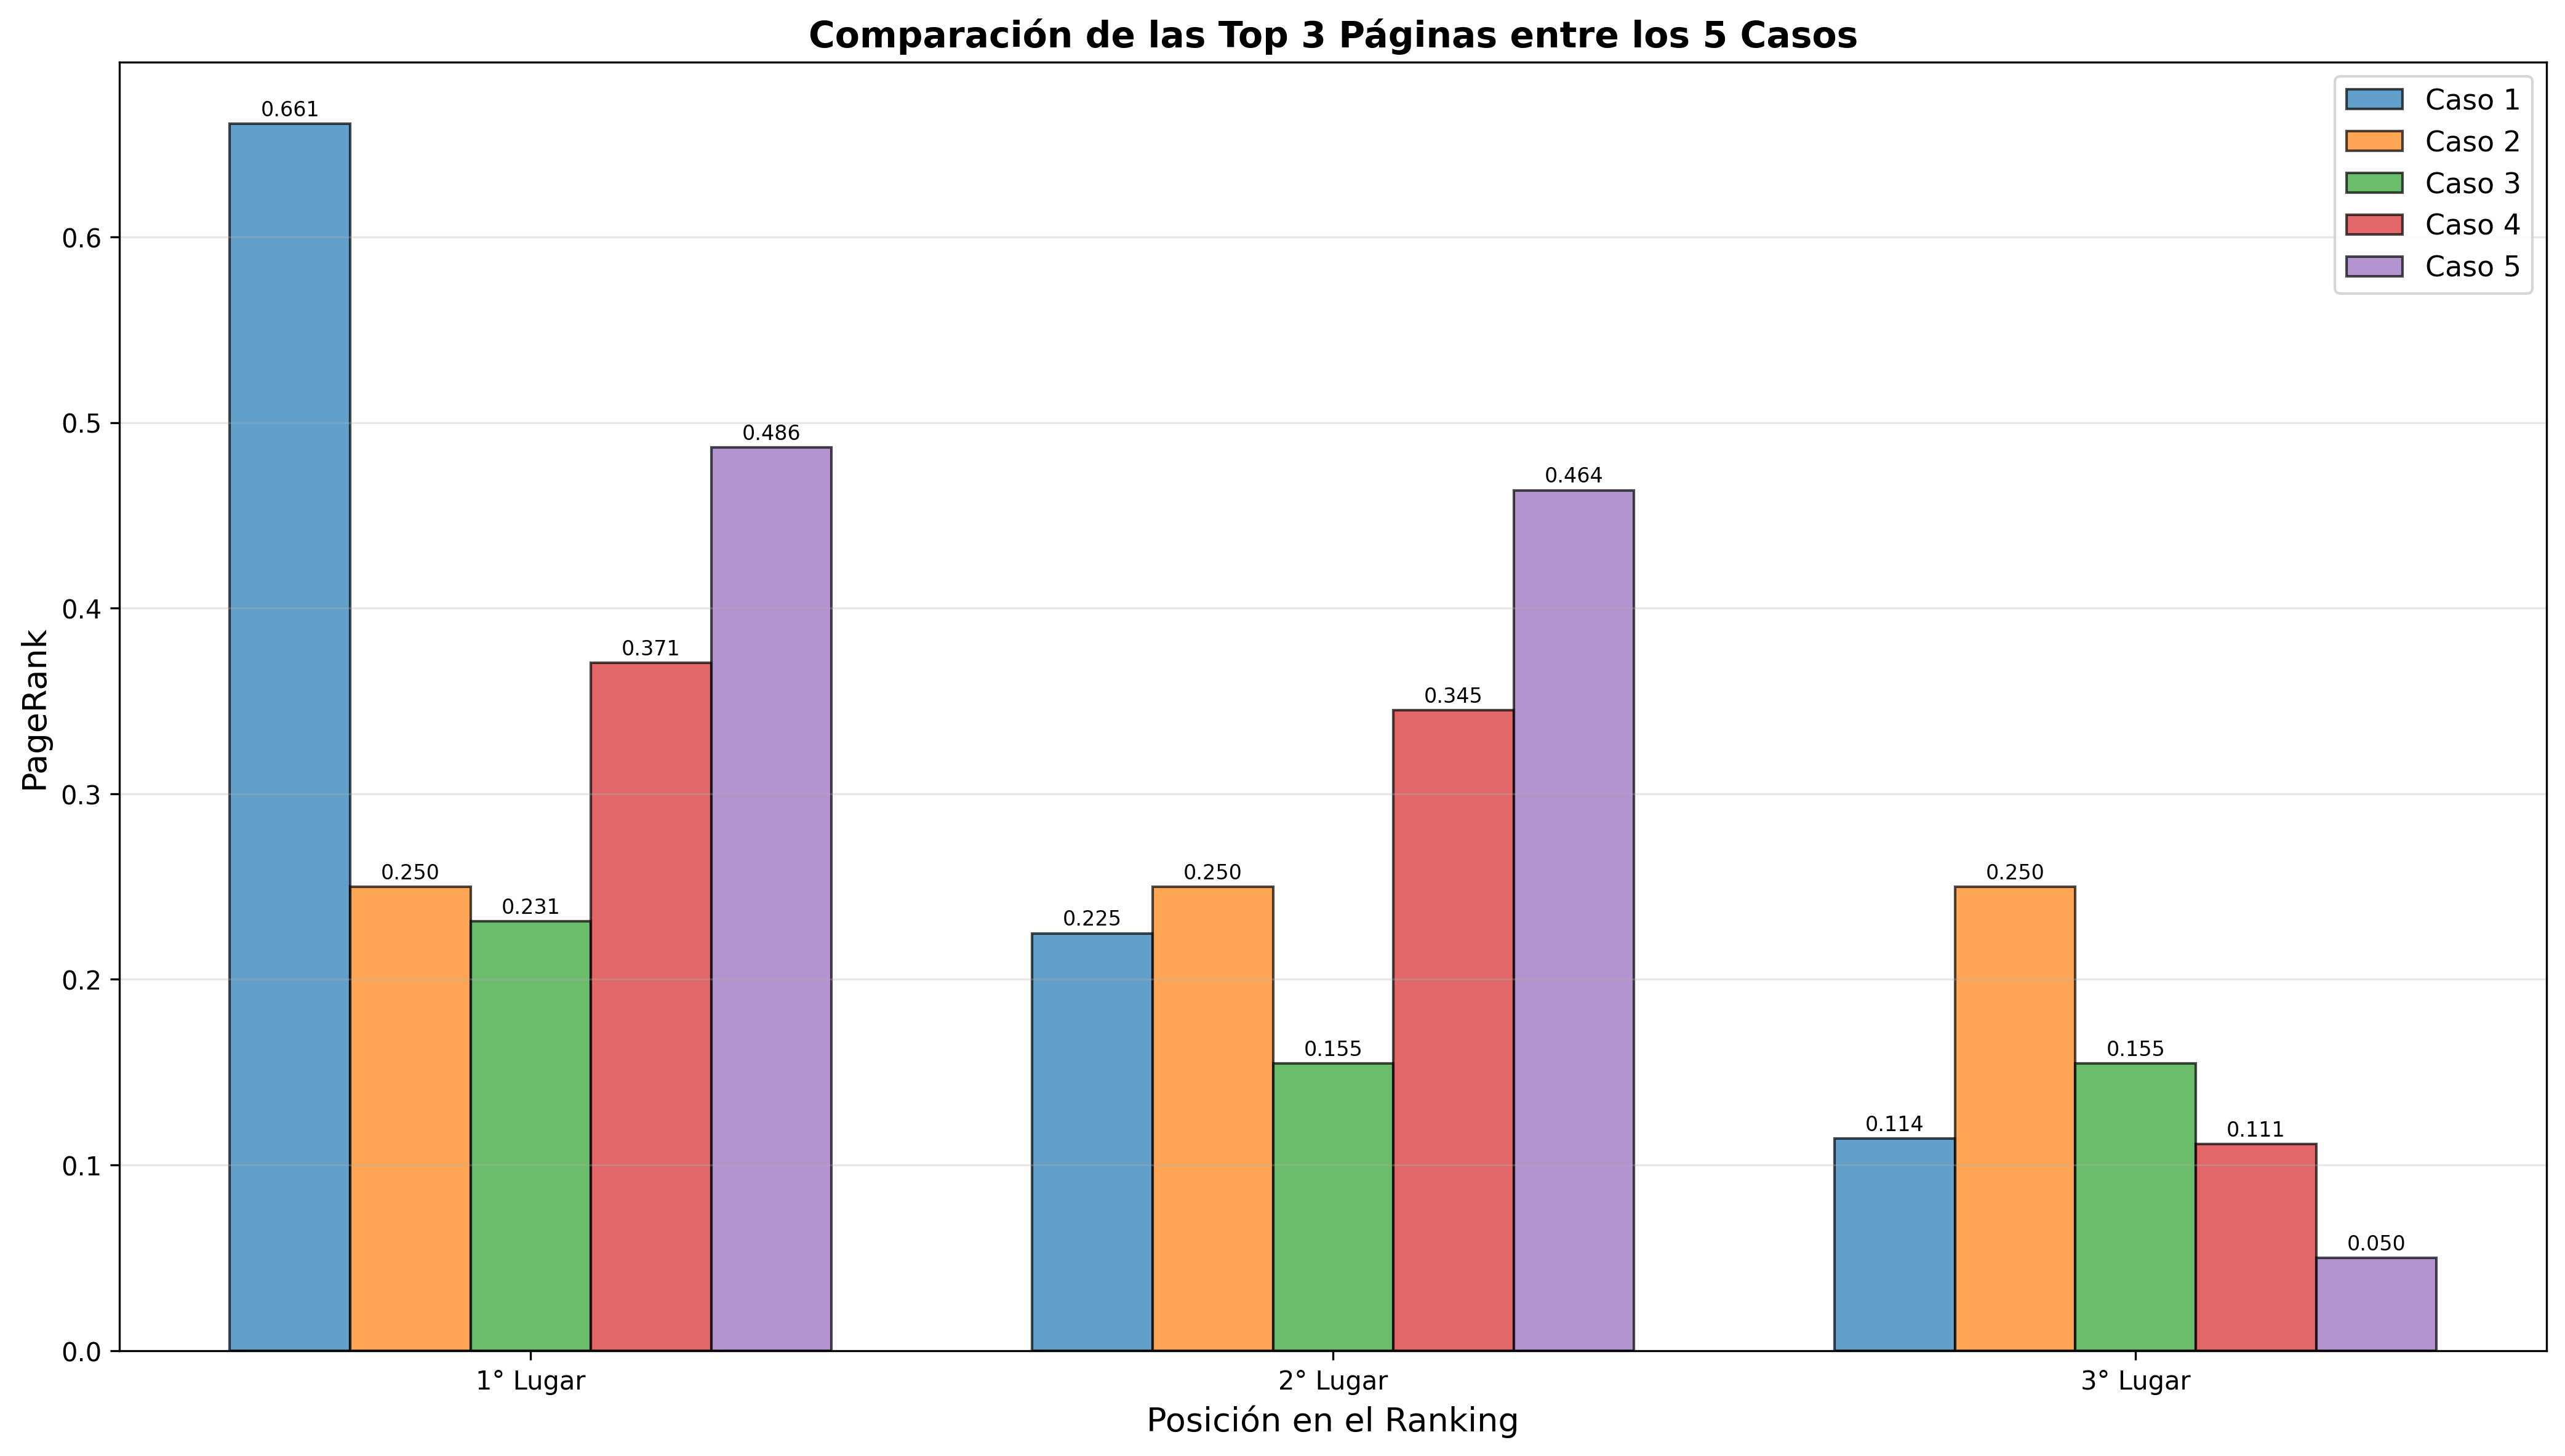
\includegraphics[width=0.9\textwidth]{../resultados/graficos/04_comparacion_top_pages.png}
    \caption{Comparación agrupada del PageRank de los 3 nodos más importantes (Top 3) a través de los 5 casos de prueba.}
    \label{fig:comparacion_top}
\end{figure}

\begin{itemize}
    \item En el \textbf{Caso 2}, la diferencia entre el 1° y el 3° lugar es nula, reflejando una red descentralizada.
    \item En los \textbf{Casos 1, 4 y 5}, se observa una pendiente negativa pronunciada entre el 1° y el 3° lugar. Esto cuantifica visualmente cómo un solo nodo (el sumidero o el hub) domina la red, mientras que la importancia de los nodos restantes decae rápidamente.
    \item Esta disparidad valida que el Método de las Potencias, junto con la Matriz de Google, responde sensitivamente a la estructura de enlaces y no asigna valores aleatorios.
\end{itemize}


\begin{figure}[H]
\centering
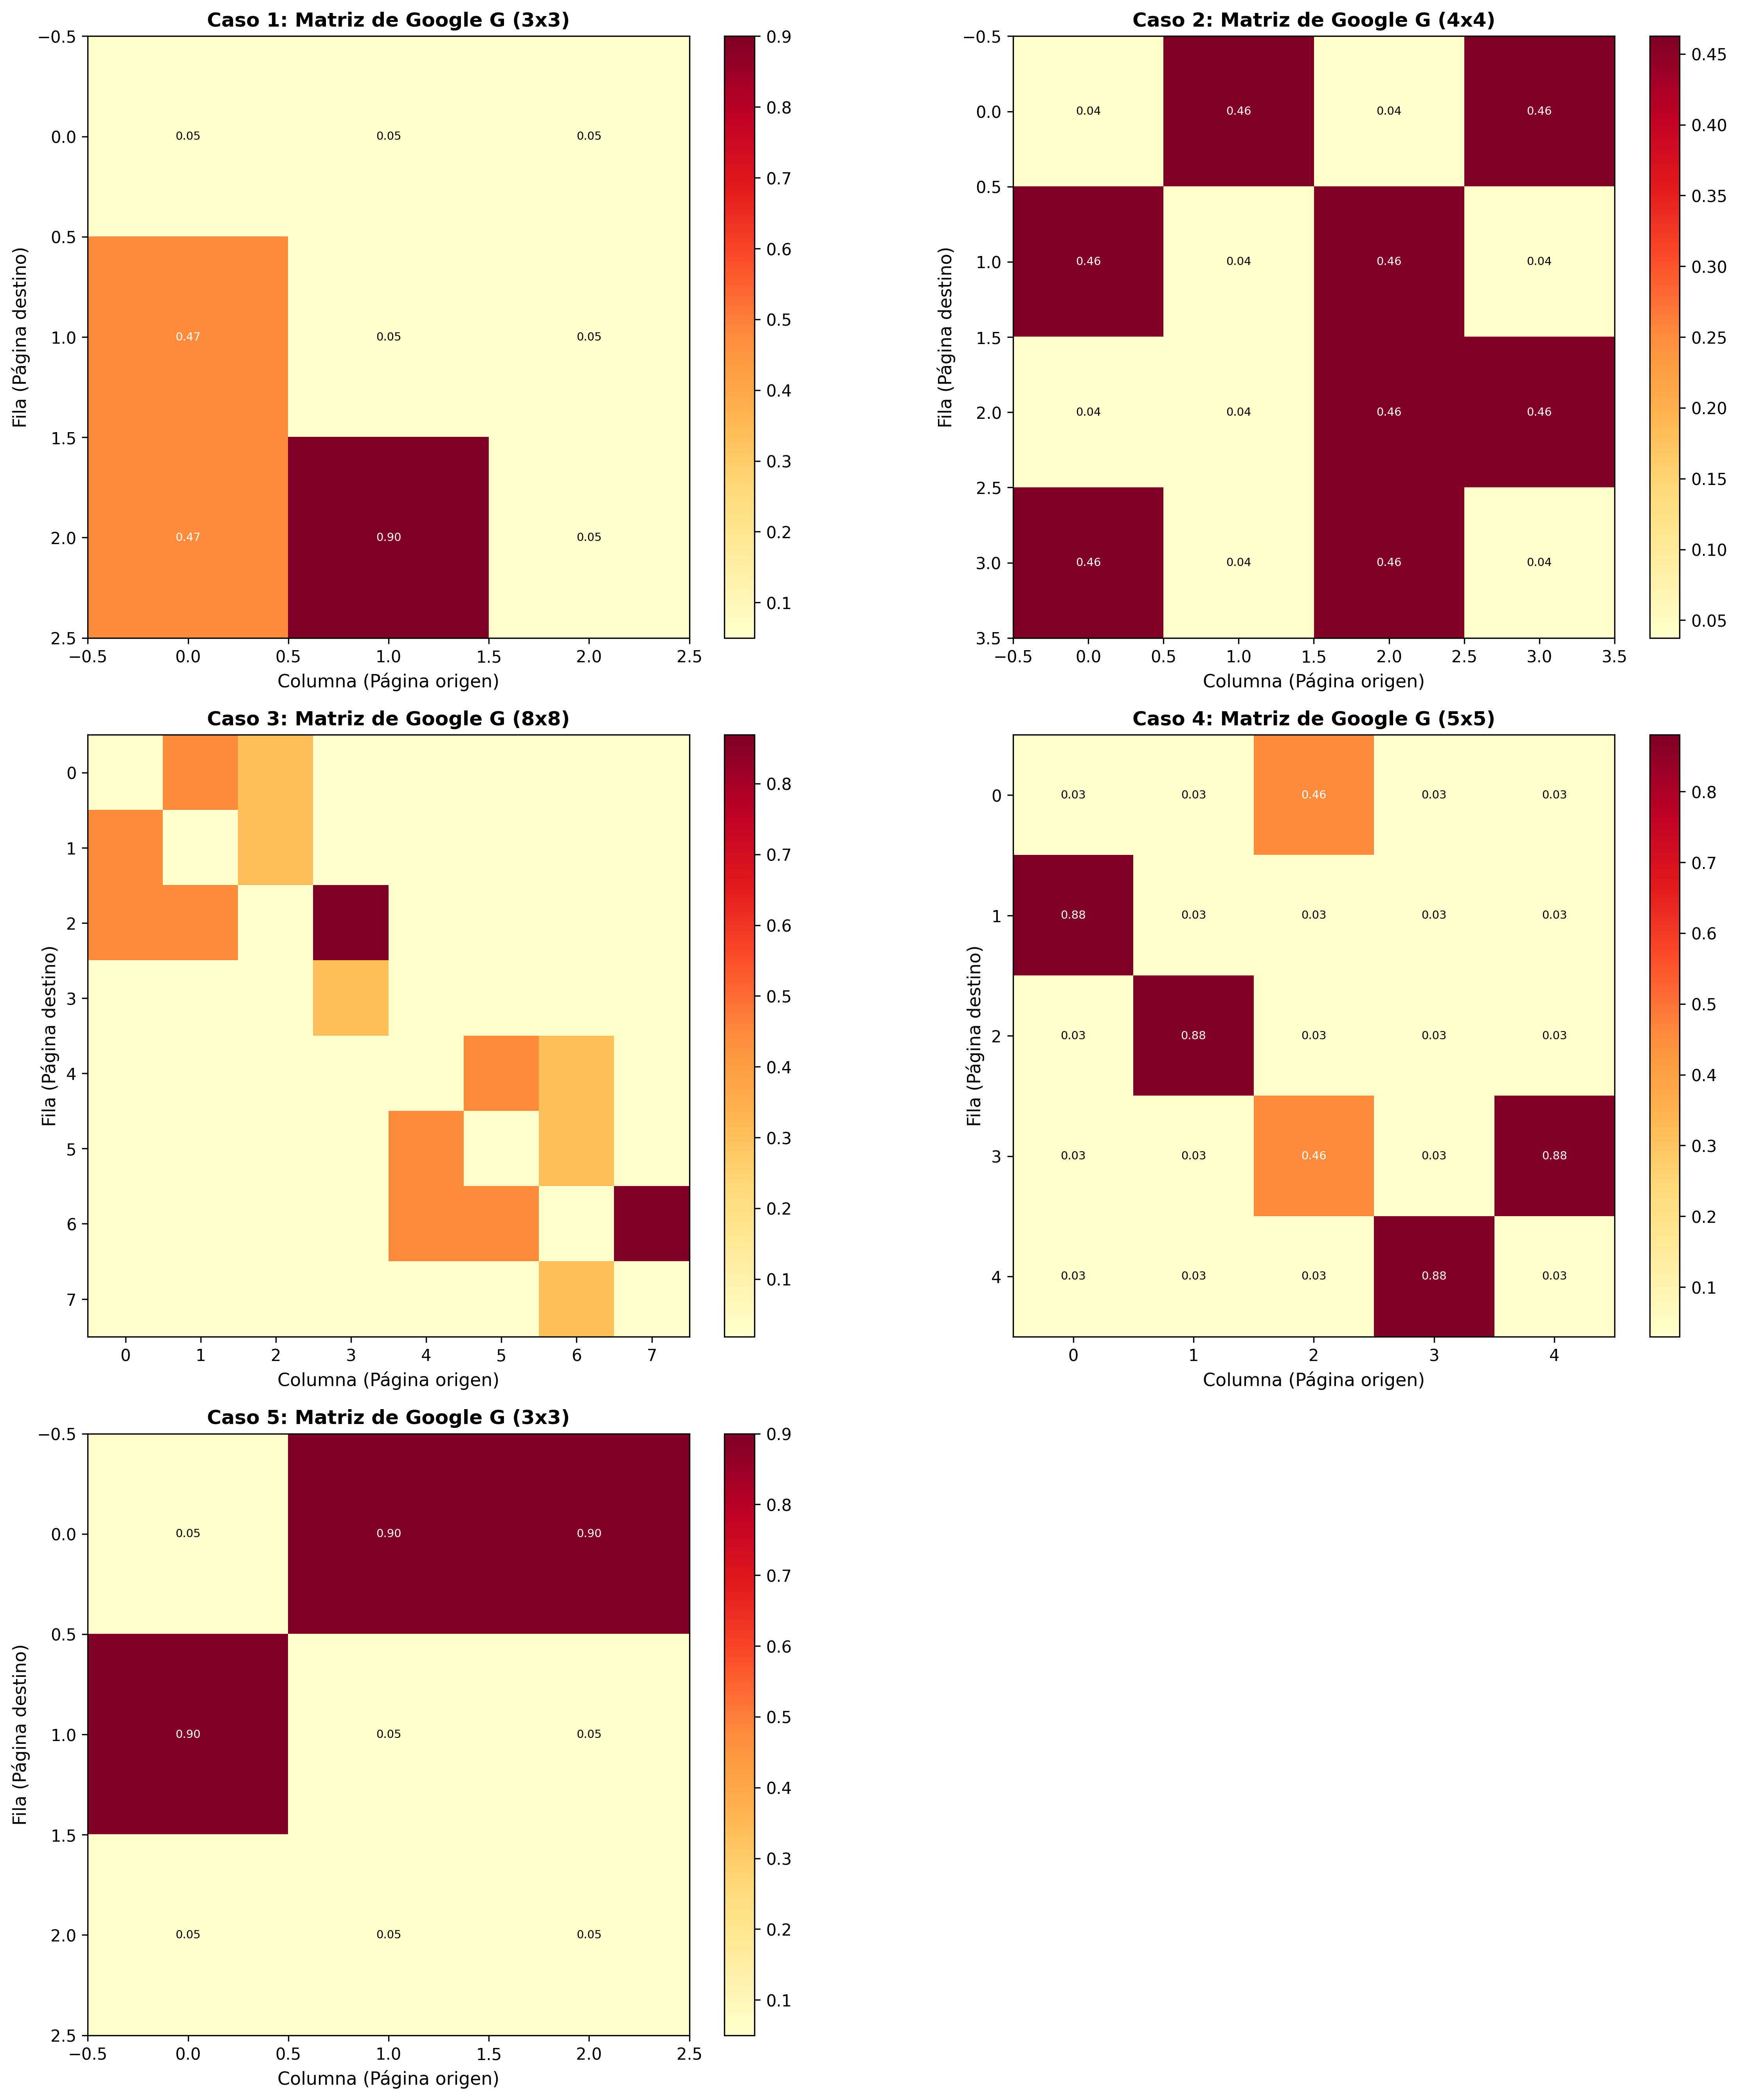
\includegraphics[width=0.9\textwidth]{../resultados/graficos/03_heatmap_matrices_G.png}
\caption{Heatmap de la Matriz de Google $G$ para el Caso 3 (8x8). Se aprecia c\'{o}mo el t\'{e}rmino $\frac{1-d}{n}$ llena la matriz con valores base (0.01875), eliminando los ceros de los sumideros.}
\label{fig:heatmap}
\end{figure}

% ---------- 5. ANALISIS FISICO ----------
\section{An\'{a}lisis Matem\'{a}tico y F\'{i}sico}\label{sec:analisis}

\subsection{Validaci\'{o}n de la Suma Unitaria}
Una propiedad fundamental del PageRank es que representa una distribuci\'{o}n de probabilidad. En todos los casos de prueba, se verific\'{o} num\'{e}ricamente que:
\begin{equation}
\sum_{i=1}^{n} v_i = 1.0 \pm 10^{-15}
\end{equation}
Esto confirma que la implementaci\'{o}n de la normalizaci\'{o}n final y la construcci\'{o}n estoc\'{a}stica de $G$ son correctas.

\subsection{Efecto del Factor de Amortiguamiento ($d = 0.85$)}
Sin el t\'{e}rmino $\frac{1-d}{n}J$, los Casos 1 y 5 habr\'{i}an fallado. El nodo sumidero habr\'{i}a atrapado todo el prestigio, y las dem\'{a}s p\'{a}ginas habr\'{i}an tendido a 0. El factor $d=0.85$ garantiza que, en cada paso, el 15\% del prestigio se redistribuya uniformemente, ``rescatando'' al sistema de los sumideros y garantizando la irreducibilidad de $G$.

\subsection{Velocidad de Convergencia}
La velocidad de convergencia del M\'{e}todo de las Potencias est\'{a} gobernada por la raz\'{o}n $\left|\frac{\lambda_2}{\lambda_1}\right| = |\lambda_2|$. 
\begin{itemize}
    \item En el \textbf{Caso 2}, $\lambda_2 = 0$, por lo que converge instant\'{a}neamente.
    \item En el \textbf{Caso 3}, la topolog\'{i}a del grafo hace que $|\lambda_2| \approx 0.98$, requiriendo 451 iteraciones para alcanzar $\epsilon = 10^{-8}$. Esto demuestra que la topolog\'{i}a de la red impacta directamente el costo computacional.
\end{itemize}

% ---------- 6. CONCLUSIONES ----------
\section{Conclusiones}\label{sec:conclusiones}

\begin{enumerate}
    \item Se implement\'{o} exitosamente el algoritmo PageRank en C++17, logrando una arquitectura modular que separa la l\'{o}gica matem\'{a}tica (Eigen) de la orquestaci\'{o}n y exportaci\'{o}n de datos.
    
    \item El uso del factor de amortiguamiento $d = 0.85$ demostr\'{o} ser crucial. Permiti\'{o} que los casos con nodos sumidero (Casos 1 y 5) convergieran correctamente, redistribuyendo el prestigio atrapado y garantizando que $G$ fuera una matriz estoc\'{a}stica positiva.
    
    \item El M\'{e}todo de las Potencias prob\'{o} ser robusto y estable, alcanzando la tolerancia de $\epsilon = 10^{-8}$ en todos los casos. Se valid\'{o} que el vector resultante siempre suma 1.0, cumpliendo con la definici\'{o}n de distribuci\'{o}n de probabilidad estacionaria de una Cadena de Markov.
    
    \item El an\'{a}lisis de los 5 casos confirm\'{o} la intuici\'{o}n f\'{i}sica del algoritmo: los nodos que reciben enlaces de otros nodos importantes, o que act\'{u}an como sumideros, acumulan mayor PageRank, mientras que los grafos regulares distribuyen el prestigio equitativamente.
    
    \item La visualizaci\'{o}n mediante Python permiti\'{o} corroborar visualmente el decaimiento exponencial del error y la estructura de la Matriz de Google, cerrando el ciclo de la metodolog\'{i}a SDD (Specification-Driven Development).
\end{enumerate}

% ---------- REFERENCIAS ----------
\begin{thebibliography}{9}

\bibitem{page1999} Page, L., Brin, S., Motwani, R., \& Winograd, T. (1999). \textit{The PageRank Citation Ranking: Bringing Order to the Web}. Stanford InfoLab.

\bibitem{langville2006} Langville, A. N., \& Meyer, C. D. (2006). \textit{Google's PageRank and Beyond: The Science of Search Engine Rankings}. Princeton University Press.

\bibitem{meyer2000} Meyer, C. D. (2000). \textit{Matrix Analysis and Applied Linear Algebra}. SIAM. (Cap\'{i}tulo sobre M\'{e}todo de las Potencias y Cadenas de Markov).

\bibitem{eigen} Eigen Documentation. \textit{Dense matrix and array manipulation}. \url{https://eigen.tuxfamily.org/dox/}

\end{thebibliography}

\end{document}